\documentclass[11pt]{amsart}

\usepackage[margin=1.15in]{geometry}
\usepackage{amsmath,amssymb,amsthm,mathtools}
\usepackage{mathrsfs}
\usepackage{bm}
\usepackage[T1]{fontenc}
\usepackage{lmodern}
\usepackage{microtype}
\usepackage{booktabs}
\usepackage{enumitem}
\usepackage{xcolor}
\usepackage{hyperref}
\setlength{\emergencystretch}{2em}
\setcounter{tocdepth}{1}

\hypersetup{colorlinks=true,linkcolor=blue!55!black,citecolor=blue!55!black,urlcolor=blue!55!black,
pdftitle={General Spectral Floors from Marked Deformation Presentations},
pdfauthor={Akari Hayami (Jian-Yu Huang)},pdfsubject={Paper III: finite marked source closure and spectral floors}}

\newtheorem{theorem}{Theorem}[section]
\newtheorem{proposition}[theorem]{Proposition}
\newtheorem{corollary}[theorem]{Corollary}
\newtheorem{lemma}[theorem]{Lemma}
\theoremstyle{definition}
\newtheorem{definition}[theorem]{Definition}
\newtheorem{remark}[theorem]{Remark}

\newcommand{\kk}{\Bbbk}
\newcommand{\Q}{\mathbb Q}
\newcommand{\im}{\operatorname{im}}
\newcommand{\kerp}{\operatorname{ker}}
\newcommand{\End}{\operatorname{End}}
\newcommand{\Hom}{\operatorname{Hom}}
\newcommand{\rankp}{\operatorname{rank}}
\newcommand{\id}{\operatorname{id}}
\newcommand{\Spec}{\operatorname{Spec}}
\newcommand{\Aeff}{\mathscr A_{\mathrm{eq}}^{\mathrm{eff}}}
\newcommand{\Aeq}{\mathscr A_{\mathrm{eq}}}
\newcommand{\Neq}{N_{\mathrm{eq}}}
\newcommand{\Geq}{\Gamma_{\mathrm{eq}}}
\newcommand{\Gmark}{\mathfrak G_{\mathrm{mark}}}
\newcommand{\Csyz}{\mathscr C_{\mathrm{syz}}}
\newcommand{\forced}{\mathrm{forced}}

\title[General Spectral Floors]{General Spectral Floors from Marked Deformation Presentations}
\author{Akari Hayami (Jian-Yu Huang)}
\date{Paper III, illustrated edition v0.09 --- September 2026}


% BEGIN ILLUSTRATION PREAMBLE
\usepackage{graphicx}
\usepackage{placeins}
\raggedbottom
\setlength{\textfloatsep}{12pt plus 2pt minus 2pt}
\setlength{\intextsep}{12pt plus 2pt minus 2pt}
\renewcommand{\topfraction}{0.9}
\renewcommand{\bottomfraction}{0.8}
\renewcommand{\textfraction}{0.08}
\renewcommand{\floatpagefraction}{0.7}
% END ILLUSTRATION PREAMBLE
\begin{document}

\begin{abstract}
We assemble a finite algebraic construction of characteristic and minimal polynomial
divisors preserved by a full normalized-tilt orbit. Chain operators supplied by a marked
relation presentation generate an effective algebra on zeroth homology. Relation seeds
then generate its smallest invariant source subspace. Together with compatible finite
state, landing, and source maps, these data determine a static normalized sector and its largest invariant core.
Without assuming invariance of the static sector, the common characteristic and minimal
polynomial divisors of the same full tilt orbit are exactly those of that core.
A finite spectral-avoidance argument proves both equalities.
Global landing descent can be weakened to local descent for the stable image;
when even local descent fails, a future-output quotient still retains well-defined dynamics.
We give explicit closure tests, an observability-kernel formula for the stable core,
and a finite closure algorithm. Exact rational models check the separate stages.
The input bookkeeping is essential: the chain-operator marking and the state,
landing, and source maps are supplied data, not consequences of a bare filtration.
The contribution is their connection to the normalized-tilt quotient; the homological
descent, invariant-subspace closure, and observability constructions are standard.
\end{abstract}
\maketitle

\tableofcontents

\section{Introduction and scope}

Paper~I~\cite{PaperI} studies a fixed cubic contraction with a substantial recurrent
spectrum. Paper~II~\cite{PaperII} shows that the normalized internal tilt orbit of its
seven-dimensional envelope retains only the divisor \(S+2\). This paper formulates
the finite mechanism behind that distinction and connects it to a marked relation
presentation.

Write \(P_\bullet\) for a bounded complex of finite-dimensional vector spaces,
concentrated in nonnegative homological degrees, and let \(\Gmark\) be a finite family
of specified chain endomorphisms. A preserved finite filtration may also be supplied;
it is needed only for the nilpotent-ideal observation in Section~\ref{sec:assembly}. Let
\(R_0:W_0\to H_0(P_\bullet)\) be a seed map. These data determine an effective algebra
and its generated seed module. To extract a spectral floor one also supplies the
finite state and observation data:
\[
\iota:H_0(P_\bullet)\hookrightarrow F,\quad
T\in\End(M),\quad \Lambda:M\to R,\quad D:R\to F.
\]
Thus the full input is the marked package
\[
\mathcal D=(P_\bullet,\Gmark,R_0;\iota,F,M,T,\Lambda,D).
\]
The stages, with their input dependencies understood, are
\begin{equation}
\begin{aligned}
(P_\bullet,\Gmark,R_0)&\longmapsto\Aeff
                  \longmapsto\Neq=\Aeff\,\im R_0,\\
(\Neq;\iota,D,\Lambda,T)&\longmapsto\Geq
                  \longmapsto(K_\infty,A_\Lambda|_{K_\infty})\\
&\longmapsto(\chi_{\forced},\mu_{\forced}).
\end{aligned}
\label{eq:pipeline}
\end{equation}
Neither \(D,\Lambda,T\) nor the marked operator family is reconstructed from a bare
complex. In particular, \emph{removing external inputs} in the historical v0.57--v0.61
notes means replacing separately declared algebras and invariant subspaces by their
generated versions, relative to this supplied data.

Homological descent and the stable-kernel computation are standard
\cite{StacksHomotopy,Kalman1963,BoydLall}. The operator family $A+\tau H$
is classical output injection, dual to state feedback.
Section~\ref{subsec:output-injection} makes the direct comparison with the
pole-shifting theorem \cite[Section~5.1, Theorem~13]{Sontag1998}.
The contribution here is the marked-source assembly that produces this
unchanged full orbit, not a new pole-assignment theorem.


% BEGIN ILLUSTRATION 1
Figure~\ref{fig:master-pipeline} displays the finite assembly with its supplied data and landing-descent hypothesis.
\begin{figure}[htbp]
\centering
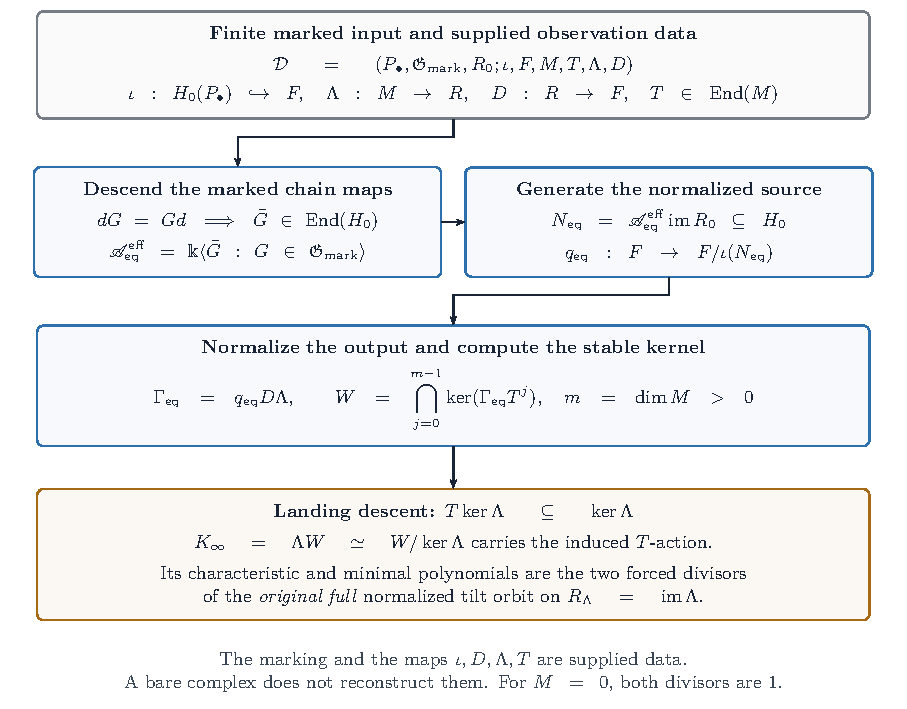
\includegraphics[width=\linewidth]{figures/fig01_master_pipeline.pdf}
\caption{The marked spectral-floor pipeline. The identification $K_\infty\simeq W/\ker\Lambda$ and its induced dynamics require $T\ker\Lambda\subseteq\ker\Lambda$. The output concerns the full original tilt orbit on $R_\Lambda=\im\Lambda$. The marking and state, source and landing maps are supplied, as in Theorem~\ref{thm:assembly}; they are not reconstructed from a bare complex.}
\label{fig:master-pipeline}
\end{figure}
\FloatBarrier
% END ILLUSTRATION 1

\section{Normalized tilts and spectral floors}

Let \(\kk\) be an infinite field, let \(R\) and \(F\) be finite-dimensional \(\kk\)-vector spaces, and let
\[
D:R\longrightarrow F, \qquad N\subseteq F, \qquad q:F\longrightarrow F/N
\]
be linear data. Define the normalized kernel
\begin{equation}
K:=D^{-1}(N),
\qquad A\in\End(R).
\label{eq:K}
\end{equation}
The allowed normalized tilts are parametrized by \(\tau\in\Hom(\im(qD),R)\), with
\begin{equation}
A_\tau:=A+\tau qD.
\label{eq:tilt}
\end{equation}
The perturbation is invisible on \(K\), so every representative has the same restriction to
\(K\).

\begin{lemma}[Exact variation space]
The set of all perturbations obtained from normalized tilts is
\begin{equation}
\{\tau qD:\tau\in\Hom(\im(qD),R)\}
=\{T\in\End(R):T|_K=0\}.
\label{eq:variation}
\end{equation}
\end{lemma}

\begin{proof}
Every \(\tau qD\) vanishes on \(K\). Conversely, if \(T|_K=0\), define \(\tau(qD r):=Tr\).
If \(qDr=qDr'\), then \(r-r'\in K\), and hence \(T(r-r')=0\). Thus \(\tau\) is well-defined
and \(T=\tau qD\).
\end{proof}

\begin{theorem}[Normalized-tilt spectral floor]
Assume \(A(K)\subseteq K\). With the characteristic and minimal polynomials of the
zero-dimensional operator both defined as \(1\), one has
\[
\mathcal O_{\mathrm{tilt}}(A)=
\{B\in\End(R):B|_K=A|_K\},
\]
and
\begin{align}
\gcd_\tau\chi_{A_\tau}&=\chi_{A|_K},\label{eq:charfloor}\\
\gcd_\tau\mu_{A_\tau}&=\mu_{A|_K}.\label{eq:minfloor}
\end{align}
The gcd is monic and is taken over the full tilt family in \eqref{eq:tilt}.
\label{thm:floor}
\end{theorem}
\begin{proof}
The orbit formula follows from the exact variation lemma. Choose \(R=K\oplus X\).
The invariance assumption and the orbit formula give precisely the matrices
\[
\begin{pmatrix} A|_K&C\\0&B_X\end{pmatrix},
\qquad C\in\Hom(X,K),\quad B_X\in\End(X).
\]
Restriction implies that \(\chi_{A|_K}\) and \(\mu_{A|_K}\) divide the corresponding
polynomial of every representative. If \(X=0\), the orbit is a singleton.

Otherwise choose two distinct scalars \(c,d\in\kk\) and take block-diagonal
representatives \(B_c=A|_K\oplus cI_X\) and \(B_d=A|_K\oplus dI_X\).
Writing \(r=\dim X\), their characteristic polynomials are
\[
\chi_{B_c}=\chi_{A|_K}(S-c)^r,\qquad
\chi_{B_d}=\chi_{A|_K}(S-d)^r,
\]
whose gcd is \(\chi_{A|_K}\). For minimal polynomials,
\[
\mu_{B_c}=\operatorname{lcm}(\mu_{A|_K},S-c),\qquad
\mu_{B_d}=\operatorname{lcm}(\mu_{A|_K},S-d).
\]
Their gcd is \(\mu_{A|_K}\), as is seen by comparing each irreducible-factor
valuation. The universal gcd divides each of these two-representative gcds,
so the lower bounds are equalities. The argument also covers \(K=0\).
\end{proof}


% BEGIN ILLUSTRATION 2
The exact variation space and two-witness argument in Theorem~\ref{thm:floor} are summarized in Figure~\ref{fig:invariant-tilt-floor}.
\begin{figure}[htbp]
\centering
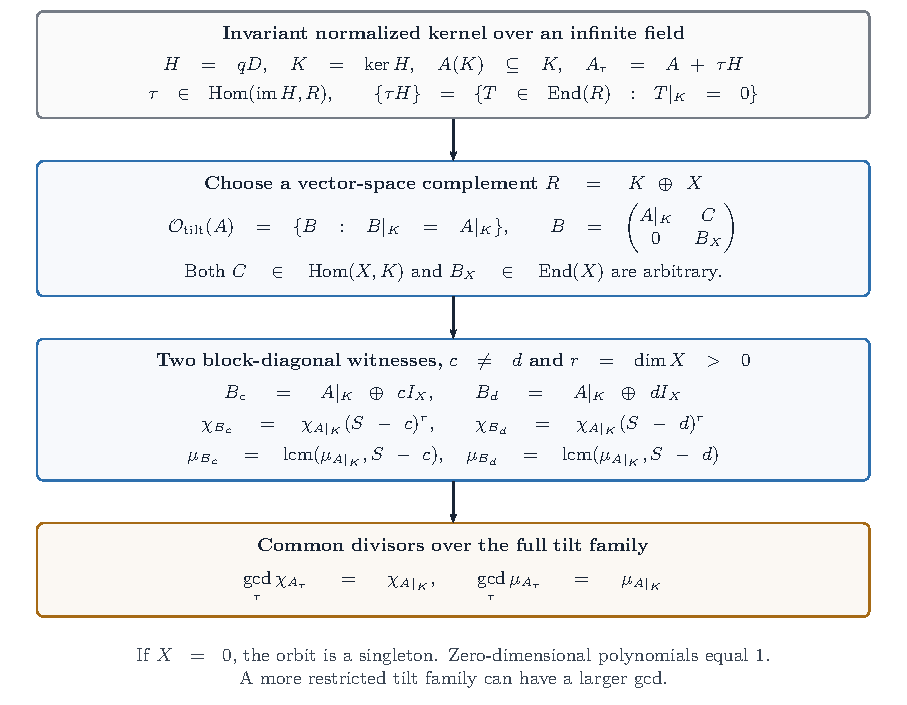
\includegraphics[width=\linewidth]{figures/fig02_invariant_tilt_floor.pdf}
\caption{The invariant normalized-tilt floor. With $K$ invariant, a chosen complement exposes arbitrary off-diagonal and quotient blocks. For a nonzero complement, two distinct scalar quotient blocks witness both monic gcds, including the case in which a scalar is a root of the forced polynomial. The zero-complement and zero-space cases use the stated conventions.}
\label{fig:invariant-tilt-floor}
\end{figure}
\FloatBarrier
% END ILLUSTRATION 2

\begin{remark}[Cubic specialization]\label{rem:cubic-specialization}
For Paper~II's internal orbit, take $R=\mathcal R$,
$A=-hD_\alpha|_{\mathcal R}$ and $H=q_FD_\alpha$.
Then $\ker H=\mathbb C E$ is invariant with $A(E)=-2E$.
Theorem~\ref{thm:floor} gives both floors equal to $S+2$, although the
selected seven-dimensional operator has a larger characteristic polynomial.
This specializes the tilt theorem; it does not supply a canonical marked
complex for the cubic equations.
\end{remark}

\begin{corollary}[Jordan-depth interpretation]
Over a splitting field, if
\[
\chi_{A|_K}(S)=\prod_\lambda(S-\lambda)^{c_\lambda},
\qquad
\mu_{A|_K}(S)=\prod_\lambda(S-\lambda)^{j_\lambda},
\]
then \(c_\lambda\) and \(j_\lambda\) are respectively the algebraic-multiplicity and
Jordan-depth floors that survive every normalized tilt.
\end{corollary}

\begin{remark}
The proof uses the full normalized variation space in \eqref{eq:variation}. If an application
restricts the tilt parameters further, the gcd can be larger. The theorem therefore identifies the
floor for the stated orbit, not for every conceivable deformation.
\end{remark}


\subsection{The same orbit without invariant normalization}\label{subsec:output-injection}

The assumption \(A(K)\subseteq K\) simplifies the answer but is not needed to
compute the floor of the original full orbit. Put \(H=qD\), \(n=\dim R>0\), and
\[
U=\bigcap_{j=0}^{n-1}\ker(HA^j).
\]
This is the usual unobservable subspace for the pair \((A,H)\)
\cite[Section~6.2]{Sontag1998}.
The nearest spectral comparison is Sontag's pole-shifting theorem
\cite[Section~5.1, Theorem~13, p.~186]{Sontag1998}: transposition converts
$A+\tau H$ to state feedback, and the fixed uncontrollable factor becomes
the characteristic polynomial on $U$. Thus the characteristic floor is
a dual output-injection consequence of that classical result.
The minimal-polynomial equality also uses a coprime block decomposition;
we prove that step below instead of attributing the equality directly
to pole assignment. Our spectral-avoidance lemma provides a self-contained
proof requiring only the weaker ability to avoid a finite spectral set.

\begin{lemma}[Avoiding a finite spectral set]\label{lem:avoidance}
Let \(B\in\End(X)\), \(C:X\to Y\), and suppose
\(\bigcap_{j\ge0}\ker(CB^j)=0\). Over an infinite field \(\kk\), for every nonzero
polynomial \(f\in\kk[S]\) there is \(L:Y\to X\) such that
\[
\gcd\bigl(\chi_{B+LC},f\bigr)=1.
\]
\end{lemma}
\begin{proof}
Work first over an algebraic closure. For any scalar \(\lambda\), the map
\(\lambda I-B\) is injective on \(\ker C\): a vector in its kernel would be
an eigenvector invisible under every \(CB^j\).
Choose \(X=\ker C\oplus X_1\). On \(X_1\), the value of \(LC\) can be prescribed
arbitrarily because \(C|_{X_1}\) is injective.
Choose these values so that the images of \(X_1\) under
\(\lambda I-B-LC\) complement \((\lambda I-B)(\ker C)\).
The resulting matrix is invertible.
Thus \(\det(\lambda I-B-LC)\), as a polynomial in the entries of \(L\),
is not identically zero for any root \(\lambda\) of \(f\).
Their finite product is nonzero, hence so is the resultant
\(\operatorname{Res}_S(f,\chi_{B+LC})\), a polynomial over \(\kk\).
A nonzero polynomial has a nonzero value at some point of an affine space over
an infinite field. That value gives the required \(L\).
The zero-dimensional and constant-\(f\) cases are immediate.
\end{proof}

\begin{theorem}[Stable-core floor for the unchanged full orbit]\label{thm:stable-floor}
For arbitrary \(A\), with no assumption that \(K=\ker H\) is invariant, \(U\)
is the largest \(A\)-invariant subspace contained in \(K\). Every representative
\(A_\tau=A+\tau H\) has the same subspace \(U\), and the same action there.
For this original tilt family,
\[
\boxed{\gcd_\tau\chi_{A_\tau}=\chi_{A|_U},\qquad
       \gcd_\tau\mu_{A_\tau}=\mu_{A|_U}.}
\]
The gcds can each be witnessed by the same two representatives.
If \(K\) is invariant, \(U=K\), recovering Theorem~\ref{thm:floor}.
\end{theorem}
\begin{proof}
Cayley--Hamilton identifies the finite intersection defining \(U\) with the
intersection over all \(j\ge0\), proving its invariance and maximality.
On any invariant subspace in \(\ker H\), \(A_\tau\) and \(A\) agree.
Applying this observation in both directions proves that the maximal such
subspace is the same throughout the orbit.

Choose \(R=U\oplus X\). Then \(A\) and \(H\) have the forms
\[
A=\begin{pmatrix}A_U&C_0\\0&B\end{pmatrix},
\qquad H=(0,C).
\]
The induced pair \((B,C)\) on \(R/U\) is observable: an invisible quotient
vector lifts to a vector in \(U\), by the infinite-intersection formula.
The quotient blocks of the original tilts range over all \(B+LC\).
Every characteristic and minimal polynomial therefore contains the respective
polynomial of \(A_U\).

By Lemma~\ref{lem:avoidance}, choose a first quotient block with characteristic
polynomial \(p_1\) coprime to \(\chi_{A_U}\), then a second with characteristic
polynomial \(p_2\) coprime to \(\chi_{A_U}p_1\).
Lift these choices to two original tilt parameters; their upper off-diagonal
blocks need not vanish. Their characteristic polynomials are
\(\chi_{A_U}p_1\) and \(\chi_{A_U}p_2\), whose gcd is \(\chi_{A_U}\).

For minimal polynomials the coprime spectra also remove the extension:
if a block-triangular operator has diagonal blocks with coprime characteristic
polynomials \(r,p\), then \(r(A)p(A)=0\), and the Bezout identity decomposes
its space as \(\ker r(A)\oplus\ker p(A)\).
The first summand is \(U\): its quotient image is zero since \(r\) is invertible
on the quotient, and \(r(A)\) vanishes on \(U\).
The other summand identifies with the quotient.
Hence for the two representatives
\[
\mu_{A_{\tau_i}}=\mu_{A_U}\,\mu_{B+L_iC},\qquad i=1,2.
\]
The two complementary minimal polynomials divide the coprime \(p_1,p_2\);
their gcd is one. This proves the minimal-polynomial equality.
If \(U=R\), the orbit is a singleton; if \(U=0\), the same argument gives
both floors equal to one. The case \(R=0\) uses the same convention.
\end{proof}

\begin{remark}
The theorem does not enlarge the allowed tilt family to all perturbations
vanishing only on \(U\). The constraints on the larger, possibly noninvariant
\(K\) remain in place. The avoidance lemma proves the upper bound within that
unchanged family.
\end{remark}


% BEGIN ILLUSTRATION 3
Figure~\ref{fig:stable-core-floor} follows the proof of Theorem~\ref{thm:stable-floor} without enlarging the allowed perturbation family.
\begin{figure}[htbp]
\centering
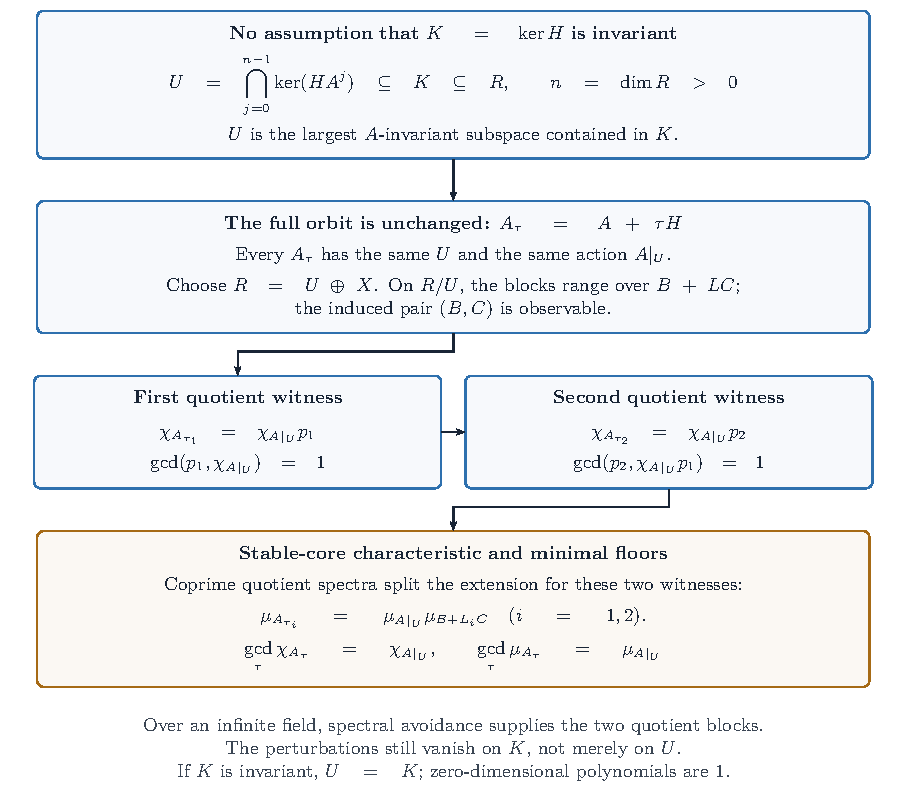
\includegraphics[width=\linewidth]{figures/fig03_stable_core_floor.pdf}
\caption{The stable-core floor without invariant normalization. Spectral avoidance over the infinite base field supplies two quotient blocks in the original orbit. Their coprime spectra also split the minimal-polynomial extension. The preserved action is on $U$, but the perturbations still vanish on the original kernel $K$.}
\label{fig:stable-core-floor}
\end{figure}
\FloatBarrier
% END ILLUSTRATION 3

\section{Forced-sector extraction from finite landing data}

Let \(M,T,\Lambda,D,F,N,q\) be finite linear data as above, and put
\[
R_\Lambda=\im\Lambda,\qquad
\Gamma=qD\Lambda,\qquad
K_\Lambda=R_\Lambda\cap D^{-1}(N).
\]
The distinction between \(R\) and \(R_\Lambda\) matters: the landing calculation
describes the visible space \(R_\Lambda\), unless \(\Lambda\) is surjective onto \(R\).

\begin{proposition}[Static extraction]\label{prop:static}
There are natural vector-space identifications
\begin{equation}
K_\Lambda=\Lambda(\ker\Gamma)
 \simeq\ker\Gamma/\ker\Lambda,\qquad
\dim K_\Lambda=\rankp\Lambda-\rankp\Gamma.
\label{eq:quotient}
\end{equation}
\end{proposition}
\begin{proof}
One has \(\Gamma m=0\) exactly when \(\Lambda m\in D^{-1}(N)\).
The kernel of \(\Lambda|_{\ker\Gamma}\) is \(\ker\Lambda\).
Apply the first isomorphism theorem and rank-nullity.
\end{proof}

\begin{proposition}[Landing descent and normalized closure]\label{prop:closure}
An operator \(A_\Lambda\in\End(R_\Lambda)\) satisfying
\(A_\Lambda\Lambda=\Lambda T\) exists uniquely if and only if
\[
T\ker\Lambda\subseteq\ker\Lambda,
\quad\text{equivalently}\quad
\rankp\begin{bmatrix}\Lambda\\\Lambda T\end{bmatrix}=\rankp\Lambda.
\]
Assuming this descent condition, \(K_\Lambda\) is \(A_\Lambda\)-invariant if and only if
\[
T\ker\Gamma\subseteq\ker\Gamma,
\quad\text{equivalently}\quad
\rankp\begin{bmatrix}\Gamma\\\Gamma T\end{bmatrix}=\rankp\Gamma.
\]
When both hold, \(A_\Lambda|_{K_\Lambda}\) is conjugate to the operator induced by \(T\)
on \(\ker\Gamma/\ker\Lambda\).
\end{proposition}
\begin{proof}
The formula \(A_\Lambda(\Lambda m)=\Lambda Tm\) is well-defined exactly under
the first kernel condition. Given it, for \(m\in\ker\Gamma\) one has
\(A_\Lambda\Lambda m\in K_\Lambda\) exactly when \(\Gamma Tm=0\).
Finally \(\ker L\subseteq\ker LT\) is equivalent to equality of the displayed
stacked rank with \(\rankp L\).
\end{proof}

\begin{proposition}[Stable core]\label{prop:stable}
Let \(m=\dim M>0\) and
\[
\mathcal O=
\begin{bmatrix}\Gamma\\\Gamma T\\ \vdots\\\Gamma T^{m-1}\end{bmatrix},
\qquad M_\infty=\ker\mathcal O.
\]
Then \(M_\infty=\bigcap_{j\ge0}\ker(\Gamma T^j)\) is the largest \(T\)-invariant
subspace contained in \(\ker\Gamma\). In general its landed image satisfies
\[
\Lambda(M_\infty)\simeq
M_\infty/(M_\infty\cap\ker\Lambda).
\]
If the landing descent condition of Proposition~\ref{prop:closure} holds, then
\(\ker\Lambda\subseteq M_\infty\) and
\[
K_\infty:=\Lambda(M_\infty)\simeq M_\infty/\ker\Lambda,\qquad
\dim K_\infty=\rankp\Lambda-\rankp\mathcal O.
\]
It is the largest \(A_\Lambda\)-invariant subspace of \(K_\Lambda\).
\end{proposition}
\begin{proof}
Cayley--Hamilton reduces every power \(T^j\), \(j\ge m\), to the first \(m\)
powers, proving the infinite-intersection equality and invariance. Any invariant
subspace in \(\ker\Gamma\) is in this intersection. The general quotient formula
is rank-nullity for \(\Lambda|_{M_\infty}\). Under landing descent,
\(\Lambda T^j n=0\) for \(n\in\ker\Lambda\), so \(n\in M_\infty\).
If \(L\subseteq K_\Lambda\) is \(A_\Lambda\)-invariant, then \(\Lambda^{-1}(L)\)
is \(T\)-invariant and contained in \(\ker\Gamma\), hence is contained in \(M_\infty\).
\end{proof}

This is the classical unobservable-subspace construction
\cite{Kalman1963,BoydLall}, used here for the normalization output \(\Gamma\).
For \(M=0\) all spaces and ranks are zero. Under landing descent,
Theorem~\ref{thm:stable-floor} identifies the floor of the original landed tilt
orbit with the operator on \(K_\infty\), even if normalized closure fails.
There is no need to replace the tilt orbit by a less constrained one.


\begin{proposition}[Local descent and the future-output quotient]\label{prop:local-descent}
Even without global landing descent, set \(W=M_\infty\) and
\(J=W\cap\ker\Lambda\). A well-defined operator on \(\Lambda W\) with
\(A_W\Lambda w=\Lambda Tw\) exists if and only if \(TJ\subseteq J\).
When it exists, it is conjugate to the action on \(W/J\).

Without that local condition, let
\[
J_{\mathrm{fut}}=\bigcap_{j=0}^{m-1}\ker(\Lambda T^j).
\]
Then \(J_{\mathrm{fut}}\subseteq W\) is invariant, and \(W/J_{\mathrm{fut}}\)
always has an induced operator. It identifies with the image of the finite
future-output map
\[
w\longmapsto(\Lambda w,\Lambda Tw,\ldots,\Lambda T^{m-1}w),\qquad w\in W.
\]
It is the smallest quotient of \(W\) preserving every future landing output:
any quotient through which all maps \(\Lambda T^j|_W\) factor has its kernel
contained in \(J_{\mathrm{fut}}\).
\end{proposition}
\begin{proof}
\(W\) is \(T\)-invariant. Thus the formula on \(\Lambda W\) is well-defined
exactly when the kernel \(J\) of \(\Lambda|_W\) is \(T\)-invariant.
Cayley--Hamilton makes \(J_{\mathrm{fut}}\) invariant and replaces its finite
intersection by the infinite one. Since \(\Gamma=qD\Lambda\), invisibility
under every \(\Lambda T^j\) implies invisibility under every \(\Gamma T^j\);
hence \(J_{\mathrm{fut}}\subseteq W\).
The first isomorphism theorem proves the finite-output identification.
The final claim is exactly the intersection-of-kernels criterion for factorization.
\end{proof}

\begin{remark}
The future-output quotient retains history, not just the static point \(\Lambda w\).
It can have larger dimension than \(\Lambda W\). It does not invent an operator
on the original static landing space when descent fails, nor does it remove
\(\Lambda\) or \(T\) from the supplied data.
\end{remark}


% BEGIN ILLUSTRATION 4
Figure~\ref{fig:landing-future} distinguishes static extraction, global descent, local descent and the future-output quotient of Proposition~\ref{prop:local-descent}.
\begin{figure}[htbp]
\centering
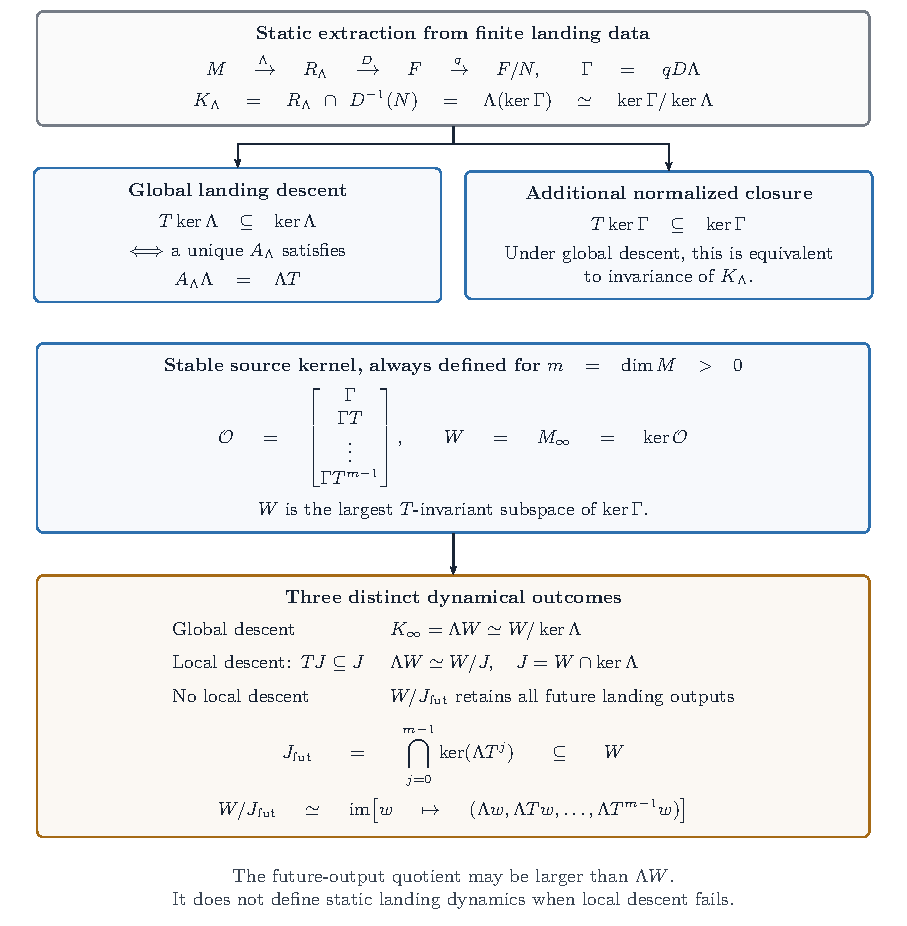
\includegraphics[width=\linewidth]{figures/fig04_landing_future_output.pdf}
\caption{Landing and retained future outputs. Static extraction is a vector-space statement. Global descent supplies the shorter stable quotient; local descent supplies dynamics only on $\Lambda W$. When local descent fails, $W/J_{\rm fut}$ is the smallest quotient preserving all future landing outputs. It can be larger than $\Lambda W$ and does not supply an operator on the original static landing space.}
\label{fig:landing-future}
\end{figure}
\FloatBarrier
% END ILLUSTRATION 4

\begin{corollary}[Cyclic polynomial module]\label{cor:cyclic}
Let \(M=\kk[S]/(c)\), with \(T\) acting by multiplication by \(S\).
Suppose both kernels are submodules and
\[
\ker\Lambda=(d_\Lambda)/(c),\qquad
\ker\Gamma=(d_\Gamma)/(c),
\]
where the displayed divisors of \(c\) are monic. Then \(d_\Gamma\mid d_\Lambda\), and
\[
K_\Lambda\simeq \kk[S]/(d_\Lambda/d_\Gamma).
\]
The characteristic and minimal polynomials of the induced cyclic operator are both
\(d_\Lambda/d_\Gamma\), with the zero-module convention equal to \(1\).
\end{corollary}
\begin{proof}
Kernel inclusion reverses divisibility of the generators. Multiplication by
\(d_\Gamma\) identifies
\(\kk[S]/(d_\Lambda/d_\Gamma)\) with
\((d_\Gamma)/(d_\Lambda)\), which is the required kernel quotient.
\end{proof}

\section{Generating the normalized source}

The normalized source should not be postulated when it can be generated from relation data. Let
\(W_{\rm rel}\) be a finite relation-seed space, let
\[
R_0:W_{\rm rel}\longrightarrow F
\]
be the seed map, and let \(C_1,\ldots,C_s\in\End(F)\) be source-side constraint propagators.
Starting from \(N^{(0)}=\im R_0\), define
\begin{equation}
N^{(r+1)}=N^{(r)}+\sum_{i=1}^s C_iN^{(r)},
\qquad
\Neq:=\bigcup_{r\geq 0}N^{(r)}.
\label{eq:closure}
\end{equation}
Because \(F\) is finite-dimensional, the increasing sequence stabilizes.

\begin{proposition}[Minimal invariant source]
The stable space in \eqref{eq:closure} is
\begin{equation}
\Neq=\kk\langle C_1,\ldots,C_s\rangle\im R_0,
\label{eq:Neq}
\end{equation}
and it is the unique smallest subspace of \(F\) that contains \(\im R_0\) and is invariant under
every \(C_i\).
\end{proposition}

\begin{proof}
Induction gives \(N^{(r)}\) equal to the span of all words in the \(C_i\) of length at most
\(r\) applied to \(\im R_0\). The stable union is therefore the right-hand side of
\eqref{eq:Neq}. Any invariant subspace containing the seed contains every such word, proving
minimality.
\end{proof}

\begin{proposition}[Functoriality]
Suppose \(\Phi_F:F\to F'\) and \(\Phi_W:W_{\rm rel}\to W'_{\rm rel}\) satisfy
\[
\Phi_FR_0=R_0'\Phi_W,
\qquad
\Phi_FC_i=C_i'\Phi_F.
\]
Then \(\Phi_F(\Neq)\subseteq N_{\rm eq}'\). If \(\Phi_F\) and \(\Phi_W\) are isomorphisms intertwining all
data, it carries \(\Neq\) isomorphically to \(N_{\rm eq}'\).
More generally, when \(\Phi_F\) is invertible, equality holds if and only if
\[
\im R_0'\subseteq\Phi_F(\Neq).
\]
In particular, mapping the seed image onto the target seed image is sufficient,
but not necessary: it suffices to generate every target seed.
\end{proposition}
\begin{proof}
The intertwining identities send every operator word applied to a seed to the
corresponding target word. This proves inclusion. With an invertible ambient map, \(\Phi_F(\Neq)\) is invariant
under every target propagator. If it contains the target seed image, minimality
gives the reverse inclusion. Conversely equality necessarily contains that image.
\end{proof}

In the source-generation step the ambient space can be the relation module itself.
If it embeds in a larger source space by \(\iota\), use \(N=\iota(\Neq)\) there.
The landed forced sector is then
\[
\Geq=q_{\rm eq}D\Lambda,\qquad
K_\Lambda\simeq\ker\Geq/\ker\Lambda,
\]
with the closure conditions of Proposition~\ref{prop:closure}. No choice of
propagators outside the embedded relation module is needed.


% BEGIN ILLUSTRATION 5
The closure construction, minimality and generated-coverage criterion are collected in Figure~\ref{fig:generated-source}.
\begin{figure}[htbp]
\centering
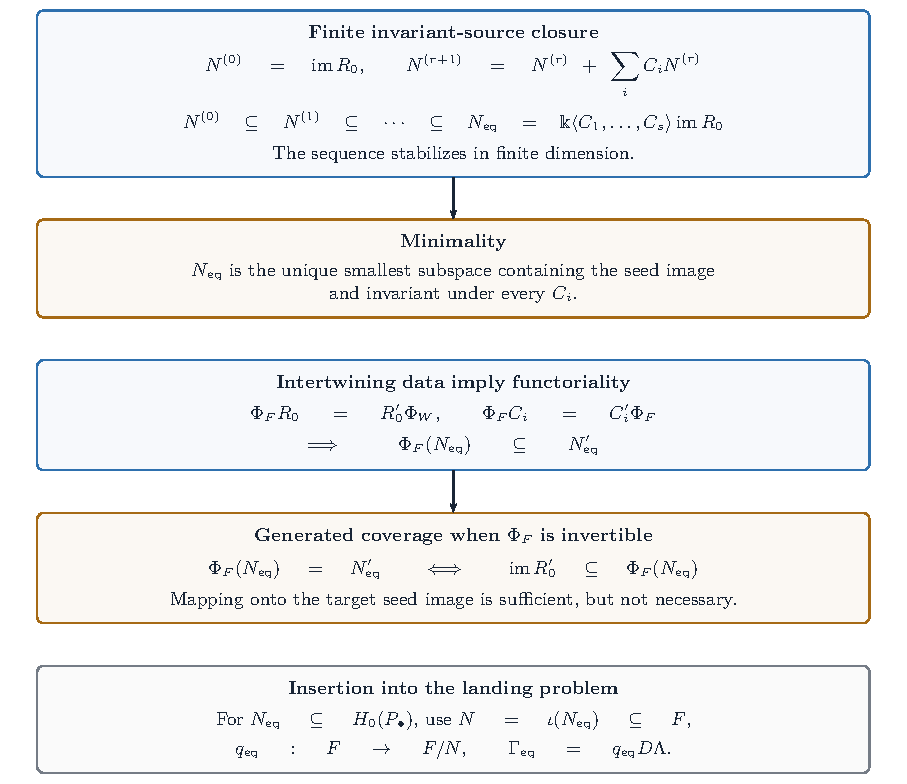
\includegraphics[width=\linewidth]{figures/fig05_generated_source.pdf}
\caption{Generating the normalized source. Intertwining maps preserve the generated source. For an invertible ambient comparison, equality is equivalent to coverage of the target seeds by the generated image; surjectivity onto the target seed image itself is not necessary. The last panel specializes to the relation module on $H_0$ and its supplied embedding into $F$.}
\label{fig:generated-source}
\end{figure}
\FloatBarrier
% END ILLUSTRATION 5

\section{Syzygies and the constraint propagator}\label{sec:syzygy}

The source propagators themselves must come from an equation action. Let \(\Aeq\) temporarily denote
a unital algebra and let \(F_{\rm rel}\) be a finite-dimensional left module. Let
\[
P_1\xrightarrow{d_1}P_0\xrightarrow{\varepsilon}F_{\rm rel}\longrightarrow 0
\]
be an exact presentation in left \(\Aeq\)-modules. Equivalently,
\(F_{\rm rel}=H_0(P_\bullet)\) for the two-term complex.

\begin{proposition}[Syzygy descent]
If \(\Aeq\) acts on the presentation complex by chain maps, it induces a representation
\(\bar\rho:\Aeq\to\End(H_0(P_\bullet))\). Let
\(\bar\varepsilon:H_0(P_\bullet)\xrightarrow{\sim}F_{\rm rel}\)
be the presentation isomorphism. The induced source constraint
propagator is
\begin{equation}
C(a)=\bar\varepsilon\,\bar\rho(a)\,\bar\varepsilon^{-1}
\quad\text{on the identified relation image},
\label{eq:Csyzygy}
\end{equation}
and the effective constraint algebra is
\begin{equation}
\Csyz=\im\bigl(C:\Aeq\to\End(F_{\rm rel})\bigr)
\simeq\Aeq/\operatorname{Ann}(F_{\rm rel}).
\label{eq:Csyz}
\end{equation}
\end{proposition}

\begin{proof}
The chain-map condition preserves \(\im d_1\), so the action on \(P_0\) descends to
\(P_0/\im d_1=H_0(P_\bullet)\). Transport along the presentation isomorphism gives
\eqref{eq:Csyzygy}. The kernel of the resulting representation is exactly the annihilator of the
relation module, which proves \eqref{eq:Csyz}.
\end{proof}

Changing generators or replacing the presentation by an isomorphic presentation complex changes matrices but
not the induced representation on \(H_0\). An ambient extension of \(C(a)\) outside the relation
image is noncanonical and has no role in \(\Neq\). This is the precise syzygy-to-propagator bridge
needed by the source-closure step.

\section{Reconstructing the effective equation algebra}

The temporary algebra $\Aeq$ in Section~\ref{sec:syzygy} is now removed
from the external input. Let $P_\bullet$ be a bounded finite-dimensional
relation complex and let
\[
\Gmark=\{G_1,\ldots,G_t\}
\]
be the specified marking. No acyclicity in positive homological degrees
is required: only the induced action on $H_0(P_\bullet)$ is used.
Assume each operator is a chain map:
\[
dG_j=G_jd.
\]
Write \(H_0=H_0(P_\bullet)\). Each \(G_j\) descends to \(\bar G_j\in\End(H_0)\).

\begin{definition}[Effective equation-operator algebra]
The effective algebra of the marked presentation is
\begin{equation}
\Aeff:=\kk\langle\bar G:G\in\Gmark\rangle
\subseteq\End(H_0).
\label{eq:Aeff}
\end{equation}
Equivalently, if \(\kk\langle X_G:G\in\Gmark\rangle\) is the free unital algebra, evaluation gives
\begin{equation}
\im(\operatorname{ev}_P)
\simeq
\kk\langle X_G:G\in\Gmark\rangle/\ker(\operatorname{ev}_P).
\label{eq:freeeval}
\end{equation}
\end{definition}

\begin{proposition}[Minimality and comparison]\label{prop:algebra-comparison}
The algebra \(\Aeff\) is the smallest unital subalgebra of \(\End(H_0)\) containing
the descended operators. Suppose the two marked families are indexed in correspondence
and a chain map \(\Phi:P_\bullet\to P'_\bullet\) satisfies
\[
\Phi G-G'\Phi=d'H_G+H_Gd
\]
for degree-one chain homotopies \(H_G:P_\bullet\to P'_{\bullet+1}\).
Then \(\bar\Phi\bar G=\bar G'\bar\Phi\) on \(H_0\). If \(\bar\Phi\) is an
isomorphism, conjugation by \(\bar\Phi\) identifies the two effective algebras.
\end{proposition}
\begin{proof}
The chain-map condition preserves boundaries, so descent is well-defined.
The homotopy equation induces equality on homology \cite{StacksHomotopy}.
Intertwining the generators intertwines every evaluated word; an invertible
\(\bar\Phi\) gives the stated conjugacy. Formula~\eqref{eq:freeeval} is the
first isomorphism theorem for the evaluation representation.
\end{proof}

A noninvertible comparison still intertwines evaluated words; an isomorphism
of effective algebras does not follow without the extra hypothesis.
Likewise, adding a contractible direct summand has no effect when the descended
marked actions are identified, even if the raw actions on the acyclic summand differ.
Transporting through the presentation identification gives
\[
\Csyz\simeq\Aeff,\qquad \Neq=\Aeff\,\im R_0.
\]
Here the first equality is a canonical identification of represented algebras,
rather than a literal equality of matrices in unrelated bases.


% BEGIN ILLUSTRATION 6
Figure~\ref{fig:syzygy-algebra} compares the syzygy action and the algebra generated by the corresponding descended marks.
\begin{figure}[htbp]
\centering
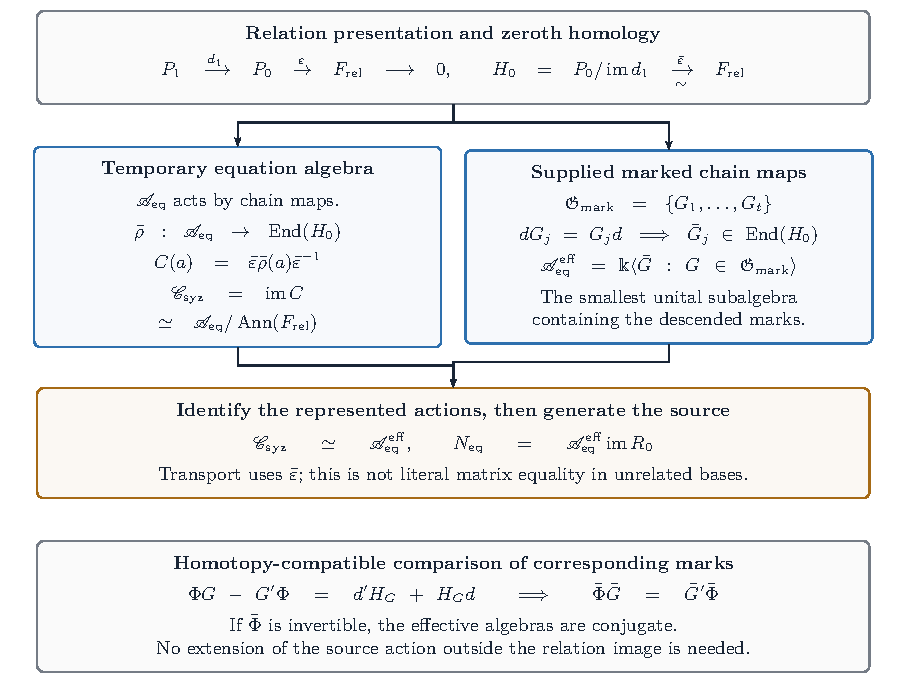
\includegraphics[width=\linewidth]{figures/fig06_syzygy_algebra.pdf}
\caption{From syzygies to the effective equation algebra. The two represented algebras are identified after transporting the same action through the presentation isomorphism. Conjugacy under a homotopy-compatible comparison requires an isomorphism on $H_0$, as in Proposition~\ref{prop:algebra-comparison}. No ambient extension outside the relation image is needed.}
\label{fig:syzygy-algebra}
\end{figure}
\FloatBarrier
% END ILLUSTRATION 6

\section{Finite closure and assembly}\label{sec:assembly}

Put \(h=\dim H_0\). Starting with \(V_0=\kk I\), form
\[
V_{j+1}=V_j+\sum_{G\in\Gmark}\bar G V_j.
\]
By induction \(V_j\) is the span of words of length at most \(j\).
Once \(V_{j+1}=V_j\), all longer words lie in the same space, so it equals \(\Aeff\).
There are at most \(h^2\) strict dimension increases; if \(h>0\) the initial
identity improves this bound to \(h^2-1\). Source closure similarly terminates after
at most \(\dim F_{\rm rel}\) strict increases. No filtration hypothesis is needed
for this termination argument.

If \(H_0=F^0H_0\supseteq\cdots\supseteq F^LH_0=0\) is a finite descending filtration
preserved by \(\Aeff\), define
\[
J=\{a\in\Aeff:a(F^pH_0)\subseteq F^{p+1}H_0\text{ for every }p\}.
\]
Then \(J\) is a two-sided ideal and \(J^L=0\): products add filtration shifts.
Thus the ideal generated by any positive-degree marked operators is nilpotent.
This conclusion requires filtration preservation by the entire represented algebra.

\begin{theorem}[Stable assembly for finite marked data]\label{thm:assembly}
Let \(\mathcal D\) be the data of Section~1. Define
\(\Neq=\Aeff\,\im R_0\subseteq H_0(P_\bullet)\),
let \(q_{\rm eq}:F\to F/\iota(\Neq)\), and put \(\Geq=q_{\rm eq}D\Lambda\).
Assume only the landing descent condition
\[
T\ker\Lambda\subseteq\ker\Lambda.
\]
For \(m=\dim M>0\), set
\[
W=\bigcap_{j=0}^{m-1}\ker(\Geq T^j).
\]
For the full original tilt family on \(R_\Lambda\), with source map
\(D|_{R_\Lambda}\) and normalization \(\iota(\Neq)\), the forced
characteristic and minimal polynomials are exactly those of the \(T\)-action on
\[
W/\ker\Lambda.
\]
If \(T\ker\Geq\subseteq\ker\Geq\), this specializes to the static quotient
\(\ker\Geq/\ker\Lambda\). For \(M=0\), both polynomials are one.
\end{theorem}
\begin{proof}
Source closure computes \(\Neq\). Landing descent defines \(A_\Lambda\).
The stable-core proposition gives \(\ker\Lambda\subseteq W\) and identifies
\(\Lambda W\) with the largest \(A_\Lambda\)-invariant subspace of
\(K_\Lambda\). Theorem~\ref{thm:stable-floor}, applied to the original family
on \(R_\Lambda\), gives the result. Under normalized closure,
\(W=\ker\Geq\), recovering the earlier static formula.
\end{proof}


% BEGIN ILLUSTRATION 7
Figure~\ref{fig:stable-assembly} separates operator closure, source closure and the stable quotient in Theorem~\ref{thm:assembly}.
\begin{figure}[htbp]
\centering
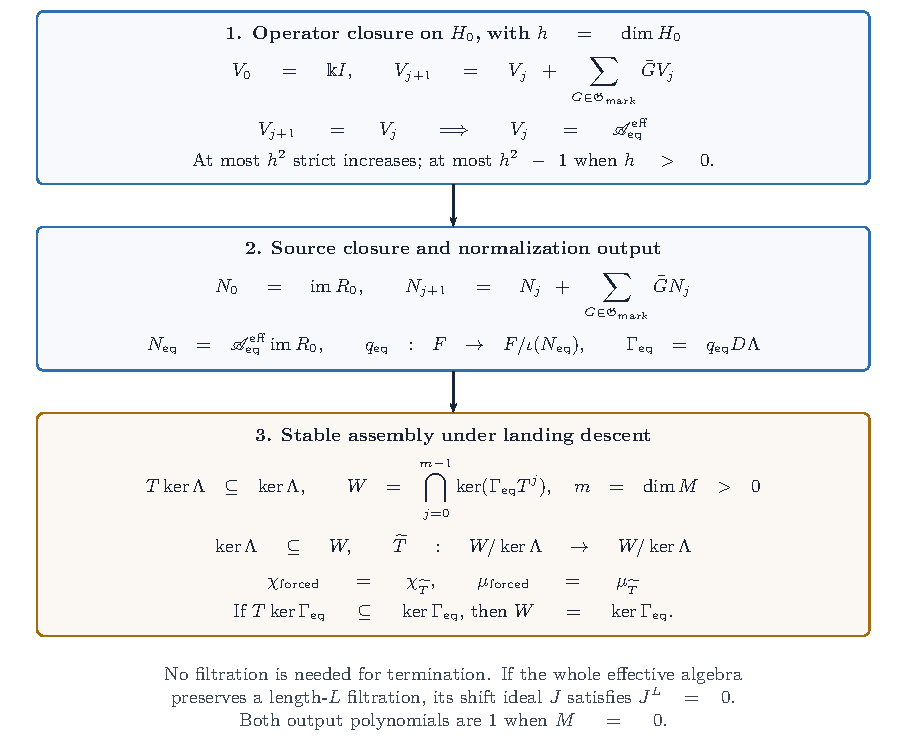
\includegraphics[width=\linewidth]{figures/fig07_stable_assembly.pdf}
\caption{Finite closure and stable assembly. The first two iterations terminate by finite dimension. Under landing descent, $\widetilde T$ is the operator induced on $W/\ker\Lambda$, and its two polynomials are the forced divisors for the unchanged full orbit. Nilpotence of the filtration-shift ideal additionally requires the whole effective algebra to preserve the filtration.}
\label{fig:stable-assembly}
\end{figure}
\FloatBarrier
% END ILLUSTRATION 7

The output is transported by isomorphisms of the full marked data: in addition
to Proposition~\ref{prop:algebra-comparison}, the seed images and the maps
\(\iota,D,\Lambda,T\) must be intertwined. Naturality of the effective algebra
alone is insufficient to compare two different landing systems.

\section{Exact finite models and verification}

\subsection{Equation-operator reconstruction model}

For this model take \(\kk=\Q\), \(H_0=\Q^4\), and
\(Se_i=e_{i+1}\) for \(i<4\), \(Se_4=0\), so \(S\) is the lower nilpotent shift, and let
\[
W=\operatorname{diag}(0,1,2,3).
\]
Then
\[
S^4=0,
\qquad
[W,S]=S.
\]
The algebra generated by \(S\) and \(W\) is the lower-triangular matrix algebra in this basis,
with dimension \(10\). Indeed the distinct diagonal weights give all four diagonal
matrix units by polynomial interpolation in \(W\), and
\(E_{ii}S^{i-j}E_{jj}=E_{ij}\) for \(i\ge j\).
The shift-only algebra \(\kk[S]\) has dimension \(4\). A change of basis
preserves these dimensions and relations after conjugation. Adding a contractible summand changes
raw chain matrices but leaves the induced \(H_0\) action unchanged. These checks verify precisely
the claims that matter for v0.61; they do not assert that arbitrary chain complexes carry such
operators canonically.

\subsection{Earlier stages of the pipeline}

The exact finite checks in the v0.57--v0.61 records \cite{PartIIIRecords}
give the following values:
\begin{table}[ht]
\centering
\caption{Exact checks for the separate finite stages.}
\label{tab:finite-checks}
\small
\begin{tabular}{@{}lll@{}}
\toprule
Version & finite output & role \\
\midrule
v0.57 & \(\chi_{\forced}=\mu_{\forced}=(S+2)^2(S-3)\), tilt dimension \(18\) & floor theorem \\
v0.58 & forced-sector dimension \(3\); cyclic floor \((S+2)^2\) & quotient extraction \\
v0.59 & ranks \(2,4,5,5\); \(\dim\Neq=5\) & source closure \\
v0.60 & syzygy rank \(4\); quotient dimension \(4\); \(\lambda^4\) & propagator bridge \\
v0.61 & \(\dim\Aeff=10\), shift-only dimension \(4\) & operator reconstruction \\
\bottomrule
\end{tabular}
\end{table}

The five historical-stage verifier scripts, together with the bundled recovery
models, are finite symbolic or exact matrix checks. Their PASS outputs are evidence
for the listed models and identities. They are not substitutes for the hypotheses in
Theorems~\ref{thm:floor} and the propositions above.


\subsection{A noninvariant normalization with an exact floor}
Take
\[
A=\begin{pmatrix}0&0&0\\0&2&0\\1&0&3\end{pmatrix},
\qquad H=\begin{pmatrix}0&0&1\end{pmatrix}.
\]
Then \(K=\ker H=\operatorname{span}(e_1,e_2)\) is not invariant, but
\(U=\operatorname{span}(e_2)\). The original orbit allows changes only to the third column.
The parameters \(\tau_0=(0,0,-3)^{\mathsf T}\) and
\(\tau_1=(-1,0,-3)^{\mathsf T}\) give
\[
\chi_{A+\tau_0H}=(S-2)S^2,\qquad
\chi_{A+\tau_1H}=(S-2)(S^2+1).
\]
These two matrices are cyclic, so their minimal polynomials are the same as
their characteristic polynomials. Both gcds are exactly \(S-2\).
The supplement also tests noncyclic Jordan cores, rational changes of basis,
multiple outputs, local descent without global descent, and generated-seed
coverage without surjectivity onto the target seed image.


% BEGIN ILLUSTRATION 8
Figure~\ref{fig:exact-floor} displays the noninvariant kernel and both rational witnesses in this example.
\begin{figure}[htbp]
\centering
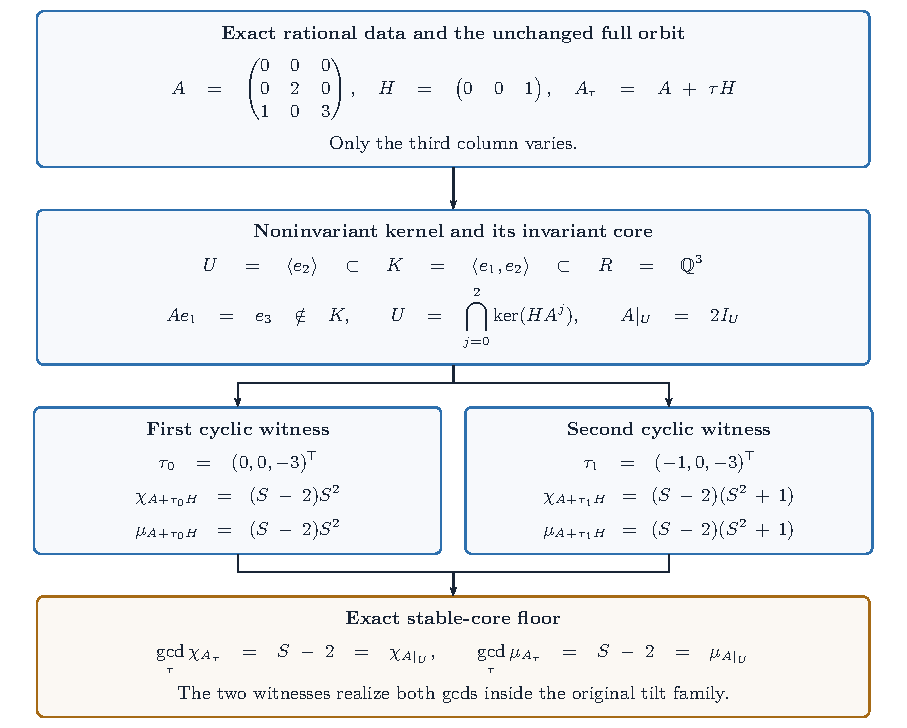
\includegraphics[width=\linewidth]{figures/fig08_exact_floor.pdf}
\caption{An exact noninvariant-normalization floor. The matrices for $\tau_0$ and $\tau_1$ are cyclic, so the displayed characteristic and minimal polynomials coincide for each witness. Their gcd is $S-2$, precisely the polynomial of the invariant core $\Q e_2$. All variations remain confined to the third column.}
\label{fig:exact-floor}
\end{figure}
\FloatBarrier
% END ILLUSTRATION 8

For an end-to-end marked realization, take
\(P_1=\Q\), \(P_0=\Q^3\), \(d_1(z)=(0,0,z)\), and mark the chain map
\(G_0=\operatorname{diag}(1,2,3)\), \(G_1=3\).
Then \(H_0(P_\bullet)=\Q^2=F\), with the identity embedding and descended
operator \(\bar G=\operatorname{diag}(1,2)\).
The seed \(R_0(s)=(s,0)\) generates \(N=\Q(1,0)\), while
\(\Aeff\) is the two-dimensional diagonal algebra.
With \(M=R=\Q^3\),
\(T=A\), \(\Lambda=I\), and
\[
D(x_1,x_2,x_3)=(0,x_3),
\]
one has \(qD\Lambda=H\). Thus every arrow of the stable assembly is realized
in one exact finite model, including a failure of normalized closure.
This is an explicit marked model, not a claim that the same inputs arise
canonically in every inverse-Leibniz presentation.


% BEGIN ILLUSTRATION 9
The supplied maps and every stage of this realization are shown together in Figure~\ref{fig:marked-realization}.
\begin{figure}[htbp]
\centering
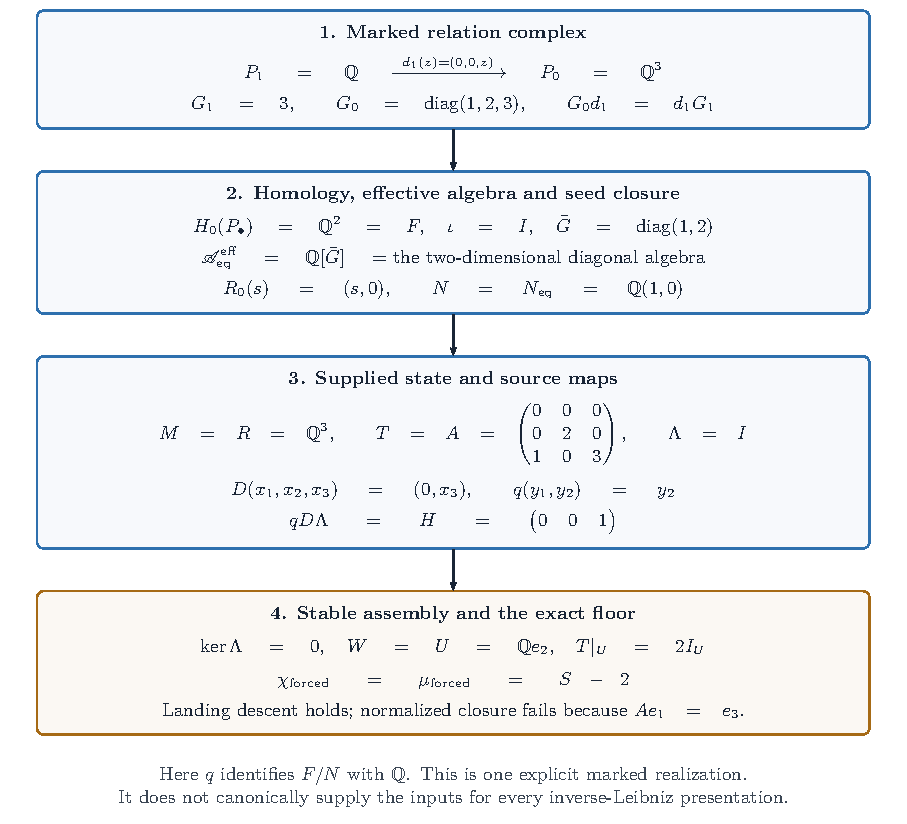
\includegraphics[width=\linewidth]{figures/fig09_marked_realization.pdf}
\caption{One complete marked realization of stable assembly. The quotient $F/N$ is identified with $\Q$ by $q(y_1,y_2)=y_2$. Landing descent holds because $\Lambda=I$, whereas normalized closure fails. The stable-core theorem still gives both floors equal to $S-2$. This finite model does not assert canonical origin of the inputs in every inverse-Leibniz presentation.}
\label{fig:marked-realization}
\end{figure}
\FloatBarrier
% END ILLUSTRATION 9

\section{Scope boundary and conclusion}

A bare complex and its filtration cannot select an arbitrary distinguished
endomorphism family. For example, take \(P_0=\Q^4\), all other \(P_i=0\), and the
descending coordinate flag preserved by lower triangular matrices. The marks
\(\{S\}\) and \(\{S,W\}\) above are both allowed on that same filtered complex,
but their generated algebras have dimensions \(4\) and \(10\). The unmarked input
does not determine which marked algebra was intended. This does not exclude
intrinsically distinguished scalar maps such as the identity, or a more restrictive
geometric construction that supplies additional operators.


% BEGIN ILLUSTRATION 10
Figure~\ref{fig:marked-scope} exhibits the two markings on the same filtered complex used in the preceding scope argument.
\begin{figure}[htbp]
\centering
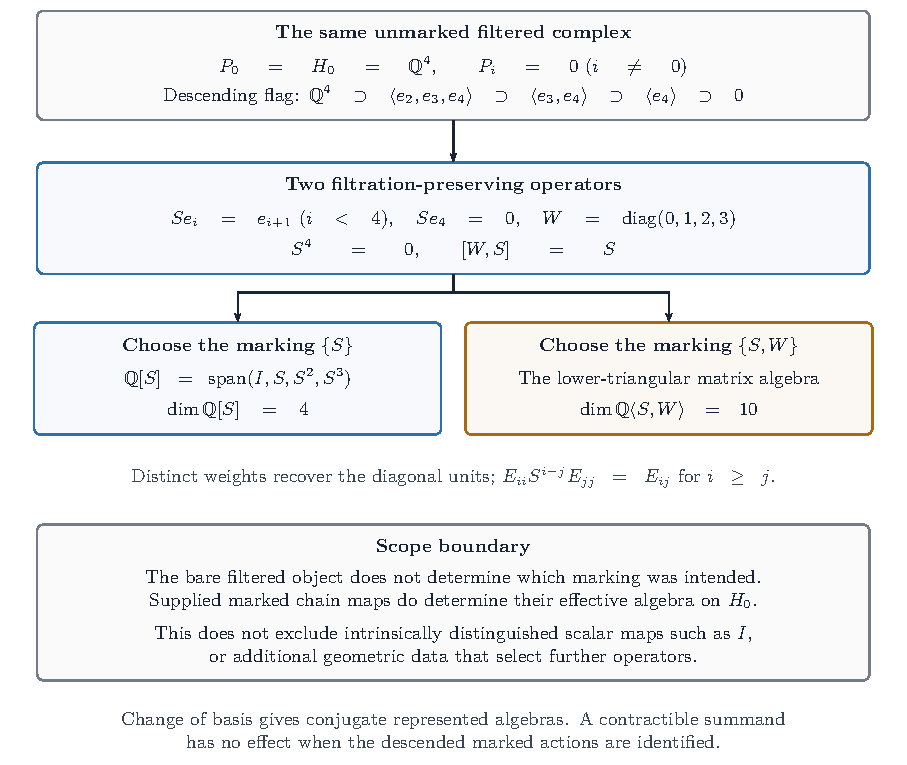
\includegraphics[width=\linewidth]{figures/fig10_marked_scope.pdf}
\caption{Marked reconstruction and its scope boundary. The shift-only and shift-plus-weight markings generate algebras of dimensions $4$ and $10$ on the same filtered object. Thus the unmarked object does not determine which marking was intended. This does not exclude scalar maps such as the identity or a more restrictive geometric construction supplying additional operators.}
\label{fig:marked-scope}
\end{figure}
\FloatBarrier
% END ILLUSTRATION 10

Within the specified marked category, the sequence v0.57--v0.61 gives a finite
assembly procedure: equation action on homology, invariant source closure,
kernel-quotient extraction, and the normalized-tilt polynomial floor.
Its hypotheses explicitly retain the chain operations and the state, landing, and
source data. The exact models establish reproducible finite checks of the stages.
They do not prove that all of those inputs arise canonically from an arbitrary
inverse-Leibniz deformation problem.



The next separate question is whether a chosen deformation presentation supplies
its operator family by a natural construction. Paper~II~\cite{PaperII} already
shows why an ordinary quasi-isomorphism class can lose boundary information.
The current theorem therefore stops at the finite marked data of
Theorem~\ref{thm:assembly}.


% BEGIN ILLUSTRATION EVIDENCE NOTE
\paragraph{Illustrated-edition supplement.}
The portable source package contains ten native vector figure masters,
the unchanged v0.57--v0.61 finite verifiers in
\path{evidence/verification/part_III/}, and the bundled v0.02/v0.03
recovery checks with their required inputs. Run \path{verify_evidence.py}
for the finite replay and \path{verify_integrated.py} for manuscript and
PDF checks. The v0.08 three-paper archive remains the broader companion;
its cited editions and the mathematical body are retained. The illustrations
summarize the proofs and finite models and do not replace them.
% END ILLUSTRATION EVIDENCE NOTE

\begin{thebibliography}{99}
\raggedright

\bibitem{PaperI}
Akari Hayami (Jian-Yu Huang),
\emph{The Inverse Leibniz Problem: Reconstruction Fibers, Rigidity, Obstructions, and Deformation DGLAs},
Paper I, illustrated edition v0.09, based on the fixed-case v0.41 record, 2026.
Unpublished companion manuscript.

\bibitem{PaperII}
Akari Hayami (Jian-Yu Huang),
\emph{Resonance-Marked Naturality and Homotopy-Tilt Non-Invariance in the Inverse-Leibniz Cubic Case},
Paper II, illustrated edition v0.09, 2026. Unpublished companion manuscript.


\bibitem{StacksHomotopy}
The Stacks Project Authors,
\emph{Homotopic maps induce the same maps on homology},
Lemma~10.71.3, Tag~00LR.
\url{https://stacks.math.columbia.edu/tag/00LR}. Accessed September 5, 2026.

\bibitem{Kalman1963}
R.~E.~Kalman,
\emph{Mathematical description of linear dynamical systems},
J. Soc. Indust. Appl. Math. Ser. A Control \textbf{1} (1963), no.~2, 152--192.
\href{https://doi.org/10.1137/0301010}{doi:10.1137/0301010}.

\bibitem{BoydLall}
S.~Boyd and S.~Lall,
\emph{Observability and state estimation},
EE263 lecture notes, Stanford University.
\url{https://ee263.stanford.edu/lectures/observ.pdf}. Accessed September 5, 2026.

\bibitem{Sontag1998}
E.~D.~Sontag,
\emph{Mathematical Control Theory: Deterministic Finite Dimensional Systems},
second edition, Texts in Applied Mathematics, vol.~6, Springer, New York, 1998.
Section~5.1, Theorem~13, p.~186: pole shifting; Section~6.2: observability.
\url{https://sontaglab.org/mct.html}.

\bibitem{PartIIIRecords}
Akari Hayami (Jian-Yu Huang),
\emph{Finite spectral-floor, source-closure, syzygy, and equation-operator records},
versions v0.57--v0.61, 2026. Unpublished computational records.
The five exact verifiers are included in
\path{three_papers_v0_08_bundle.zip}, under
\path{evidence/legacy/verification/part_III/}.
See \path{EVIDENCE_MAP.md} for the stage-to-file mapping and the
additional stable-core and local-descent checks. No public archive
identifier has been assigned in this local version.
\end{thebibliography}

\end{document}
